\begin{figure}[htbp]
    \captionsetup[subfigure]{justification=centering}
    \centering
    \begin{subfigure}[b]{0.3\textwidth}
        \centering
        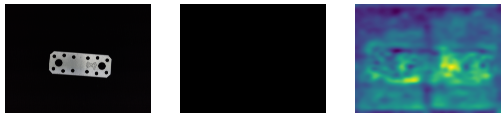
\includegraphics[width=\textwidth]{figures/ensemblehierarchyimages/image_prediction_018.png}
        %\caption*{Logical Anomalies}

    \end{subfigure}
    \begin{subfigure}[b]{0.3\textwidth}
        \centering
        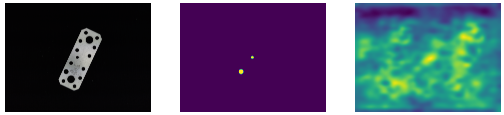
\includegraphics[width=\textwidth]{figures/ensemblehierarchyimages/image_prediction_021.png}


    \end{subfigure}
    \begin{subfigure}[b]{0.3\textwidth}
        \centering
        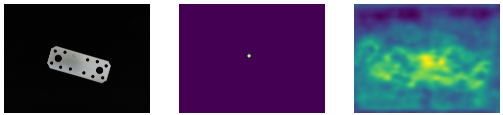
\includegraphics[width=\textwidth]{figures/ensemblehierarchyimages/image_prediction_047.png}


    \end{subfigure}
    \begin{subfigure}[b]{0.3\textwidth}
        \centering
        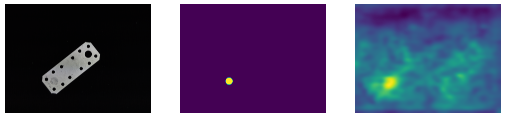
\includegraphics[width=\textwidth]{figures/ensemblehierarchyimages/image_prediction_064.png}
        %\caption*{Structural Anomalies}

    \end{subfigure}
    \begin{subfigure}[b]{0.3\textwidth}
        \centering
        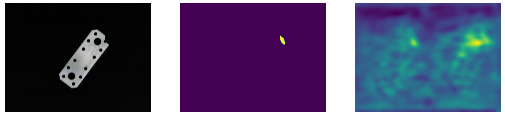
\includegraphics[width=\textwidth]{figures/ensemblehierarchyimages/image_prediction_071.png}


    \end{subfigure}
    \begin{subfigure}[b]{0.3\textwidth}
        \centering
        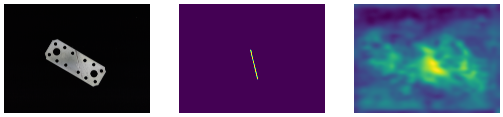
\includegraphics[width=\textwidth]{figures/ensemblehierarchyimages/image_prediction_089.png}


    \end{subfigure}
    \caption{Representative segmentation results from our stacking ensemble with multiple Wideresnet50 backbones at the various hierarchy level. The predictions are done on the novel flat 
             connector class.}
    \label{fig:ensemblehierarchy}
\end{figure}